% Five-slide overview of the DuQuantum cat-qubit results (team Shunya). Build: xelatex -interaction=nonstopmode duquantum_short.tex
\documentclass[aspectratio=169,11pt]{beamer}
\usefonttheme{professionalfonts}
\usepackage{fontspec}
\usepackage{unicode-math}
\usepackage{booktabs}
\setsansfont{FiraSans}[Path=fonts/, Extension=.otf, UprightFont=*-Regular, ItalicFont=*-Italic,
  BoldFont=*-SemiBold, BoldItalicFont=*-SemiBoldItalic]
\setmathfont{FiraMath-Regular.otf}[Path=fonts/]
\graphicspath{{../plots/}{figs/}}

\definecolor{ink}{HTML}{1F2430}
\definecolor{muted}{HTML}{5B6270}
\definecolor{accent}{HTML}{136F63}
\setbeamercolor{normal text}{fg=ink,bg=white}
\setbeamercolor{structure}{fg=accent}
\setbeamercolor{frametitle}{fg=ink}
\setbeamerfont{frametitle}{size=\Large,series=\bfseries}
\setbeamersize{text margin left=1.1cm,text margin right=1.1cm}
\setbeamertemplate{navigation symbols}{}
\setbeamertemplate{frametitle}{%
  \vspace*{0.9em}{\usebeamerfont{frametitle}\insertframetitle}\par
  \vspace{0.3em}{\color{accent}\rule{2.4em}{1.6pt}}\vspace{0.2em}}
\setbeamertemplate{footline}{%
  \hspace{1.1cm}{\color{muted}\fontsize{7}{8}\selectfont DuQuantum 2026 \quad Alice \& Bob cat qubit challenge \quad Team Shunya}%
  \hfill{\color{muted}\fontsize{7}{8}\selectfont\insertframenumber}\hspace{1.1cm}\vspace{0.45cm}}

\newcommand{\aside}[1]{{\color{muted}\footnotesize #1}}
\newcommand{\fig}[1]{\includegraphics[width=\linewidth,height=0.62\textheight,keepaspectratio]{#1}}

\begin{document}

{\setbeamertemplate{footline}{}
\begin{frame}[plain]
\begin{columns}[c]
\begin{column}{0.44\textwidth}
{\color{accent}\footnotesize\bfseries DUQUANTUM 2026 \quad ALICE \& BOB}\\[1.4em]
{\fontsize{26}{30}\selectfont\bfseries Cat qubits, simulated}\\[0.8em]
{\large How a cat qubit is made, how well it keeps its bit, and how it is read}\\[2.4em]
{\color{muted}Team Shunya}
\end{column}
\begin{column}{0.52\textwidth}
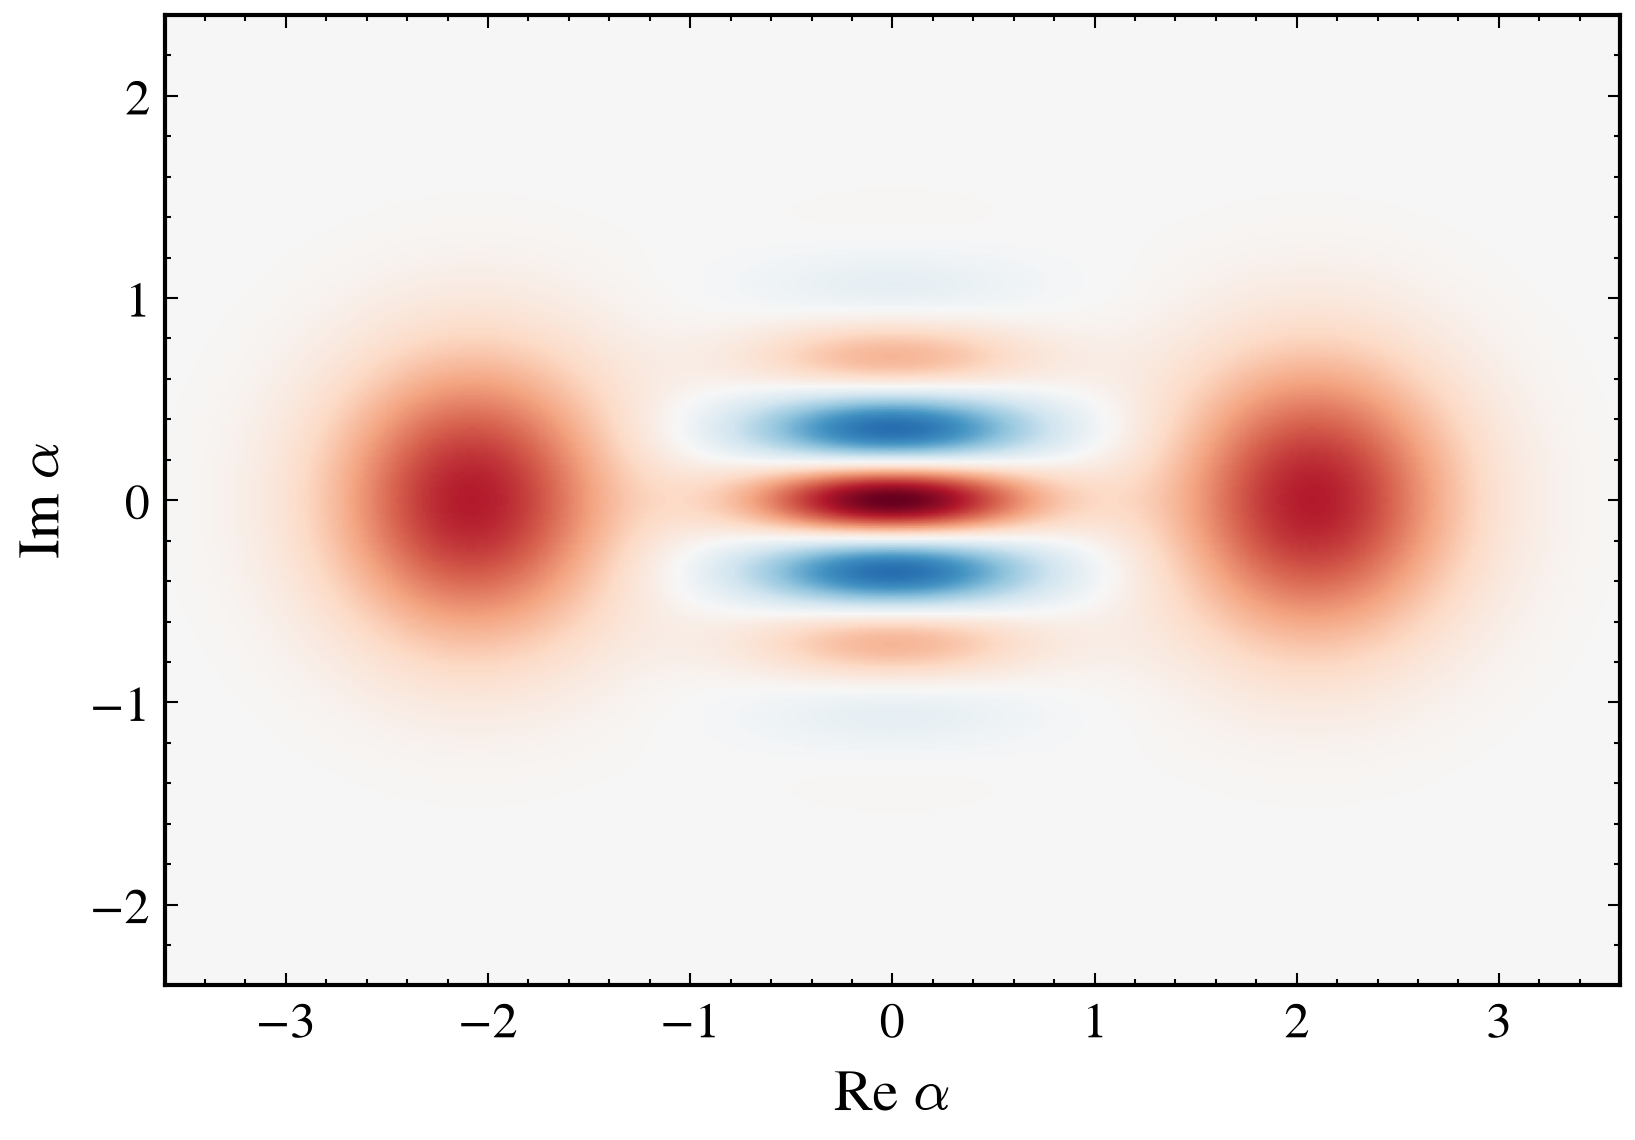
\includegraphics[width=\linewidth]{fig_cat.png}\\[0.2em]
\aside{A cat state: one resonator oscillating two opposite ways at once}
\end{column}
\end{columns}
\end{frame}}

\begin{frame}{A cat qubit is protected against one of the two errors}
\begin{columns}[c]
\begin{column}{0.42\textwidth}
\small
Qubits make two kinds of mistakes: bit flips, where 0 turns into 1, and phase flips.

\medskip
A cat qubit stores 0 and 1 as two opposite oscillations of one microwave resonator. A pump keeps pushing it back to those two states.

\medskip
Bit flips become very rare, so only phase flips are left to correct.
\end{column}
\begin{column}{0.54\textwidth}\centering
\fig{task1_1_photon_number.png}\\
\aside{Switching on the pump fills the resonator to 4.4 photons within about 1~µs.}
\end{column}
\end{columns}
\end{frame}

\begin{frame}{Bigger cats flip far less often}
\begin{columns}[c]
\begin{column}{0.42\textwidth}
\small
Each point is the bit-flip rate from one simulation, for a cat of a given size.

\medskip
The line falls steeply: for small cats, each extra photon makes bit flips about 20 times rarer.

\medskip
Phase flips grow only in proportion to the photon number, so a bigger cat is a good trade.
\end{column}
\begin{column}{0.54\textwidth}\centering
\fig{task2_1_gamma_x.png}\\
\aside{Bit-flip rate (log scale) against photon number}
\end{column}
\end{columns}
\end{frame}

\begin{frame}{At our working point a bit flip takes seconds}
\vfill
\begin{columns}[c]
\begin{column}{0.30\textwidth}\centering
{\color{ink}\Huge\bfseries 2.6 s}\\[0.4em]{\color{muted}average time to a bit flip}
\end{column}
\begin{column}{0.30\textwidth}\centering
{\color{ink}\Huge\bfseries 1.94 µs}\\[0.4em]{\color{muted}average time to a phase flip}
\end{column}
\begin{column}{0.30\textwidth}\centering
{\color{accent}\Huge\bfseries $\sim10^{6}$}\\[0.4em]{\color{muted}how much rarer bit flips are}
\end{column}
\end{columns}
\vfill
\centering\aside{A cat of 4.4 photons, simulated with both resonators and no thermal noise}
\vfill
\end{frame}

\begin{frame}{The partner resonator tells us which state the cat is in}
\begin{columns}[c]
\begin{column}{0.42\textwidth}
\small
A small push on the cat makes the partner's output go up for one state and down for the other. It settles within 1~µs.

\medskip
The push also causes a few flips, so the best readout error is about 0.4\%. Growing the cat during the readout cuts that error 13 to 18 times.

\medskip
\aside{Code and every number: github.com/\\yubrajbhandari923/DuQuantum, branch ak-changes}
\end{column}
\begin{column}{0.54\textwidth}\centering
\fig{task2_3_b_trace.png}\\
\aside{Output signal for the two states over time}
\end{column}
\end{columns}
\end{frame}

\end{document}
